\chapter{Holes in history space and their arithmetic activation}\label{ch:topology}

When does the history complex $K_A$ of a SELECT-II piece have a two-dimensional hole, and how does divisibility of the source switch it on and off? This is the central arithmetic discovery of the programme: \emph{divisibility acts on topology}. The method is certificate-based. A hole is exhibited by a pair (cycle, cocycle), and survival along the divisibility filtration is decided by which three-dimensional cells are present.

\section{Cycles, cocycles and what can change \texorpdfstring{$H_2$}{H2}}
Let $X=K_A$ with cellular chains $C_j(X)$ over $\F$ spanned by the $j$-faces and boundary $\partial_j$ (the boundary of an ordered partition is the sum of the refinements splitting one block into an ordered pair $(S|T)$). A $2$-\emph{cycle} is $z\in C_2$ with $\partial_2z=0$; a $2$-\emph{cochain} is a linear functional $\varphi$ on $C_2$.
@@def:certificate@@
@@lem:certificate@@
Since $\beta_2=f_2-\rho_2-\rho_3$ and $\partial_3$ maps $3$-faces to $2$-faces, $\beta_2$ depends only on faces of dimension $\le3$ (\cref{thm:face-threshold}(c)). Along the filtration a class created by new $2$-faces therefore survives until new $3$-faces enlarge the image of $\partial_3$ enough to kill it.
@@prop:H2-low@@

\section{The anchor cycle}
The two \emph{anchor contents} are $\lambda_A=(2,3,4,5,8,9)$ at source $288$ and $\lambda_B=(2,3,6,7,8,9)$ at source $432$. In rank coordinates $0,\dots,5$ they carry the \emph{same} combinatorial certificate.
@@def:anchor@@
The following finite facts are the combinatorial content; the full listing of $z$ and of the objects below is in \cref{app:certs}.
@@lem:PS0+computer-assisted@@
@@RAW:ch06.tex::For a content $\lambda$ put $K_z(\lambda)::$D(3)=7$.@@

\section{Parametric hole survival}
@@thm:hole-survival+analytic given the finite lemma@@
@@prop:existence-survival@@
@@thm:anchor+survival analytic, fillings finite-exact@@

\begin{figure}[ht]\centering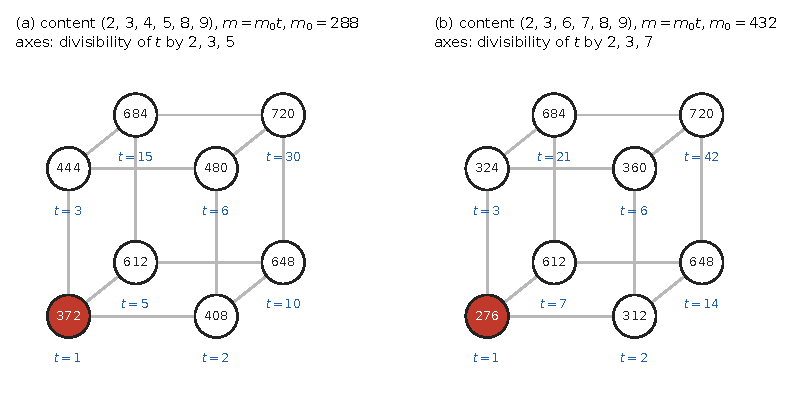
\includegraphics[width=\textwidth]{figures/fig_activation_cube.pdf}
\caption{The eight regimes of the comparable window form a Boolean cube indexed by which gate primes divide $t$ in $m=m_0t$, with history counts $N$ (exact). The hole of the anchor survives only at the bottom vertex $t$ coprime to the gate primes (red); multiplying by any gate prime fills it, and the filled state is absorbing under divisibility. Left: $\lambda_A$, $m_0=288$, gates $2,3,5$. Right: $\lambda_B$, $m_0=432$, gates $2,3,7$, where the vertex for $3\cdot7$ carries the interaction $+24$ of \cref{obs:counting}.}\label{fig:cube}
\end{figure}
\begin{figure}[ht]\centering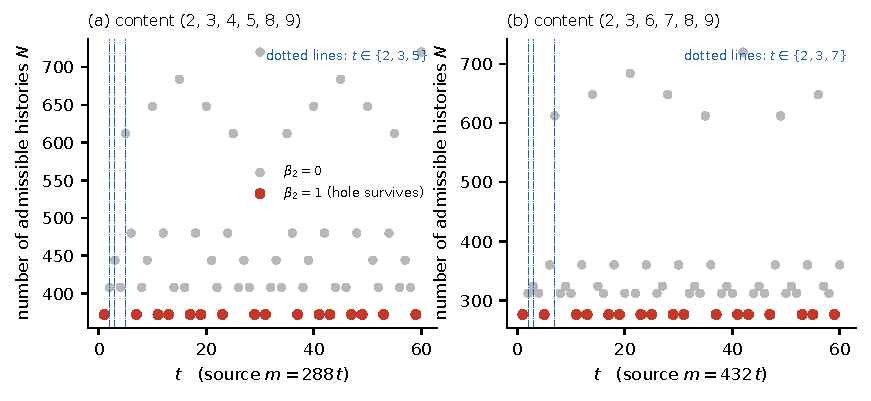
\includegraphics[width=\textwidth]{figures/fig_activation_series.pdf}
\caption{Divisibility activation along $m=288t$ and $m=432t$, $t=1,\dots,60$: the history count $N$ (exact, from the admissible-set simulation) with the sources at which the hole survives in red. Survival occurs exactly for $t$ coprime to $30$ (a) and to $42$ (b); dotted lines mark the gate primes at which a gate opens and the hole is filled.}\label{fig:activation}
\end{figure}

\section{The exact survival criterion}
\Cref{thm:hole-survival} is a sufficient condition phrased through gates. All $3$-faces of $P_6$ have $\Pref(F)\subseteq P_z\cup\mathrm{EXTRA}$, where $\mathrm{EXTRA}$ is a set of $20$ further prefix sets (listed in \cref{app:certs}). Whether $z$ bounds in $X_\lambda(m)$ with $K_z\mid m$ therefore depends only on $S=\mathfrak F_\lambda(m)\cap\mathrm{EXTRA}$, and is a monotone Boolean function of $S$: more feasible sets give more $3$-faces.
@@thm:exact-survival+finite-exact@@
@@rem:gate-correction@@
@@prop:gate-nec+finite-exact@@
@@prop:CRT@@

\section{The six-label census}
@@obs:census-H2+finite-exact@@
This is a statement about a census. It does not say that the census exhausts the mechanisms of $H_2$ (\cref{ch:atlas}), nor that labels $\le16$ exhibit gate necessity (they do not, by \cref{prop:gate-nec}). The \emph{role-permutation} caveat is essential: the identity role map (the cycle placed on ranks as given) detects only some regimes, and applying $\sigma\in S_6$ to the cycle gives different families, so a count for the ``anchor class'' must say which role maps it ranges over (see also \cref{obs:rolemap}).
